\section{Computational illustrations and training selection}
\label{sec:numerical}
The numerical study addresses two questions: how factor coordinates relate to computational geometry, and how training selection allocates fitted effects between common and sparse residual components. Six synthetic samples, one per scenario, provide fixed inputs for these illustrations. Curvature and stationarity diagnostics address the first question; three-fold validation and final-model summaries address the second.

\subsection{Synthetic design and comparison protocol}
\label{subsec:cohort-design}
Each cohort has $n=120$ training patients, $p=300$ molecular covariates, and $d=2$ clinical covariates. Independently generate the coordinates of $\bm{f}_i\in\mathbb R^2$, $\bm v_i\in\mathbb R^p$, and $\bm{Z}_i\in\mathbb R^2$ from $\operatorname{Unif}[-\sqrt3,\sqrt3]$. For $j=1,\ldots,p$, let
\begin{equation}
\begin{gathered}
\bm B_{j\cdot}=\sqrt\rho
 \left(\cos\frac{2\pi(j-1)}p,\ \sin\frac{2\pi(j-1)}p\right),\\
\bm u_i=\sqrt{1-\rho}\,\bm v_i,\qquad
\bm X_i=\bm B\bm f_i+\bm u_i.
\end{gathered}
\label{eq:pilot-design}
\end{equation}
The ordinary-model signal is $\eta_i=\bm{Z}_i^\top\bm{\theta}_0+\bm{X}_i^\top\bm{\beta}_0$, with $\bm{\theta}_0=(0.35,-0.25)^\top$ and nonzero $\bm{\beta}_0$ entries $(0.6,-0.6,0.5,-0.5,0.4)$ at indices $(1,61,121,181,241)$. All remaining entries are zero. The error is standard normal, $a_3 t_3$, or $a_C C$ with $C$ standard Cauchy, where
\[
 a_3=\Phi^{-1}(0.75)/F_{t_3}^{-1}(0.75),\qquad
 a_C=\Phi^{-1}(0.75).
\]
Thus the error interquartile ranges (IQRs) agree. Independently draw $V_i\sim N(0,1)$ and set
\begin{equation}
 \begin{gathered}
\log T_i=\eta_i+\varepsilon_i,\\
 \log C_i=\eta_i+c+V_i,
 \\
 \int F_\varepsilon(c+v)\phi(v)\,\mathrm{d}v=1-\pi_C.
 \end{gathered}
 \label{eq:pilot-censoring}
\end{equation}
Equation~\eqref{eq:pilot-censoring} calibrates the population censoring proportion $\pi_C$. Realized event indicators follow the generated event and censoring times, retaining sample variation in censoring. Computation remains on the log-time scale.

\begin{table}[htbp]
\centering\small
\caption{Synthetic-design scenarios. The error scales match interquartile ranges}
\label{tab:scenarios}
\begin{tabular}{@{}lrrl@{}}
\toprule
Scenario & $\rho$ & Target censoring & Error distribution \\
\midrule
S1 & 0 & 30\% & Standard normal \\
S2 & 0.25 & 30\% & Standard normal \\
S3 & 0.75 & 30\% & Standard normal \\
S4 & 0.75 & 30\% & IQR-scaled $t_3$ \\
S5 & 0.75 & 60\% & IQR-scaled $t_3$ \\
S6 & 0.75 & 30\% & IQR-scaled Cauchy \\
\bottomrule
\end{tabular}
\end{table}


The factor-adjusted estimator (FA) uses $K=2$ and the unadjusted estimator (UA) uses $K=0$; the loss, molecular penalty, and bandwidth $h=0.2$ agree. S1 is the prespecified over-adjustment control, with $\rho=0$. At the fixed coefficients, signal variance is approximately $1.565$, $1.3254$, and $0.8462$ for $\rho=0,0.25,0.75$. The scenarios therefore vary dependence at fixed coefficients, with the corresponding change in signal variance.

\subsection{Active curvature and work to common accuracy}
\label{subsec:geometry-results}
Both estimators use non-restarted FISTA at $\lambda=0.01$, initialized from their respective $\lambda=0.025$ fits on S3, S4, and S6. Each method retains its original parameter coordinates and training design. The common stopping threshold is $10^{-7}$ for the complete KKT residual plus the tracked numerical budget.

Factor adjustment reaches the common accuracy levels with fewer gradient evaluations in these three samples (Figure~\ref{fig:geometry-gradients}). At $10^{-6}$, first-crossing counts for FA and UA are 2,549 and 33,195 in S3, and 3,021 and 34,693 in S4. S6 FA reaches this level at 4,843 evaluations; S6 UA remains above it at its endpoint. At the prescribed $10^{-7}$ stopping level, FA takes 3,619, 3,271, and 4,507 accepted updates. UA reaches its 30,000-update limit with residuals $4.269\times10^{-7}$, $3.033\times10^{-7}$, and $2.686\times10^{-6}$. The accepted-update view is provided in Supplementary Appendix~\ref{app:reproducibility}.

For each saved endpoint, form the active set from all unpenalized coordinates and the exactly nonzero molecular coefficients. The local loss Hessian is
\begin{equation}
 \bm{H}(\bm{\vartheta})=\frac1{Nh}\sum_{i\ne j}\Delta_i
   \phi\{r_{ij}(\bm{\vartheta})/h\}\,\bm{w}_{ij}\bm{w}_{ij}^\top.
 \label{eq:geometry-hessian}
\end{equation}
We analyze $\bm{H}_{\mathcal A\mathcal A}$ using the numerical rank threshold
\[100\epsilon_{\rm mach}|\mathcal A|\max_j|\lambda_j(\bm{H}_{\mathcal A\mathcal A})|.\]
All six active Hessians were numerically full rank under this rule.
\begin{table}[htbp]
\centering\small
\caption{Active loss-Hessian spectra at the FISTA endpoints. Ratios use the smallest numerical positive eigenvalue}
\label{tab:geometry-spectrum}
\begin{tabular}{@{}llrrrr@{}}
\toprule
Scenario & Method & Dimension & Minimum & Maximum & Ratio \\
\midrule
S3 & FA & 103 & $9.055\times10^{-4}$ & 2.893 & $3.195\times10^{3}$ \\
S3 & UA & 101 & $1.055\times10^{-3}$ & 89.074 & $8.445\times10^{4}$ \\
S4 & FA & 101 & $2.188\times10^{-3}$ & 2.888 & $1.320\times10^{3}$ \\
S4 & UA & 100 & $1.508\times10^{-3}$ & 94.353 & $6.256\times10^{4}$ \\
S6 & FA & 102 & $4.942\times10^{-4}$ & 3.704 & $7.494\times10^{3}$ \\
S6 & UA & 104 & $2.463\times10^{-4}$ & 115.830 & $4.702\times10^{5}$ \\
\bottomrule
\end{tabular}
\end{table}


The spectral differences are driven primarily by the upper end: FA reduces the maximum active curvature from 89--116 to 2.89--3.70, with smaller active spectral ratios in all three samples (Table~\ref{tab:geometry-spectrum}). Minimum curvature varies by scenario and is slightly lower for FA in S3. The corresponding final scalar steps are $1/4$ for FA and $1/256$ for UA. UA's inverse step remains $L=256$ throughout its last 5,000 updates, with no further backtracking. The lower upper-curvature scale is therefore consistent with the larger scalar steps used by FA.

The largest endpoint residual lies in a nonzero molecular coefficient for all six fits. Exactly zero coordinates satisfy the KKT inequalities at the endpoints and selected late checkpoints. Across UA updates 26,000, 27,000, 28,000, 29,000, and 30,000, the saved supports and signs agree while the dominant residual coordinate changes. Clinical-block residuals also exceed $10^{-7}$ for S3 and S6 UA, confirming the need for full-coordinate accuracy.

Weak-curvature directions explain where the remaining stationarity error lies. The ten smallest-eigenvalue directions contain 79.1\%, 80.3\%, and 52.8\% of the squared active residual for S3, S4, and S6 UA. FA residuals also concentrate in weak directions. For UA, this concentration combines with a wider active spectrum and a fixed scalar step, producing small late objective ranges alongside oscillating KKT residuals. These comparisons use each method's own endpoint, active set, and optimization domain.


\begin{figure}[p]
 \centering
 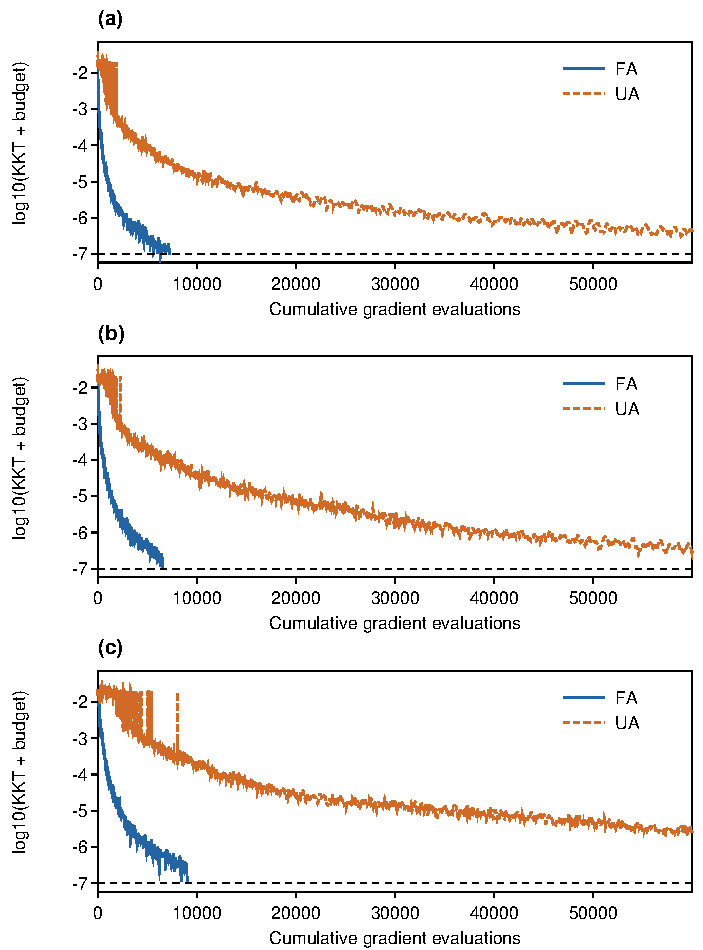
\includegraphics[width=119mm]{figures/Fig1.pdf}
 \caption{Computational work to a common stationarity tolerance. The full original-coordinate KKT residual plus its tracked numerical budget is plotted against cumulative gradient evaluations for S3, S4, and S6 in panels (a), (b), and (c). FA is solid and UA is dashed. Both methods use non-restarted FISTA, $h=0.2$, $\lambda=0.01$, and their respective $\lambda=0.025$ starts. The horizontal line is $10^{-7}$. Curves end at their FISTA stopping points, before the local refinement in Section~\ref{subsec:polish-results}}
 \label{fig:geometry-gradients}
\end{figure}

\FloatBarrier

\subsection{Active-face refinement resolves late-stage residuals}
\label{subsec:polish-results}
One active-face Newton step brings each UA endpoint below $10^{-7}$ while preserving its design, support, signs, $h=0.2$, and $\lambda=0.01$ (Table~\ref{tab:polish-results}). All three FA endpoints meet the same accuracy threshold before refinement and return unchanged.
\begin{table}[htbp]
\centering\small
\caption{Full original-coordinate KKT residuals for one-step refinement of the UA fits}
\label{tab:polish-results}
\begin{tabular}{@{}lrrr@{}}
\toprule
Scenario & Before & After & Newton updates \\
\midrule
S3 & $4.269\times10^{-7}$ & $4.864\times10^{-10}$ & 1 \\
S4 & $3.033\times10^{-7}$ & $1.780\times10^{-10}$ & 1 \\
S6 & $2.686\times10^{-6}$ & $6.997\times10^{-9}$ & 1 \\
\bottomrule
\end{tabular}
\end{table}

\FloatBarrier
All three step lengths were one, with no backtracking halvings. The full steps preserved every active molecular sign and left all original zero coefficients at zero. The new minimum inactive-coordinate margins were approximately $7.75\times10^{-5}$, $2.76\times10^{-6}$, and $9.99\times10^{-6}$. The objective decreases were approximately $2.58\times10^{-10}$, $1.02\times10^{-10}$, and $4.94\times10^{-9}$. Thus substantial reductions in full stationarity residual were obtained without changing the support or statistical objective.

The full steps provide a direct computational counterpart to the spectral diagnosis: local direction-specific scaling completes stationarity on each existing active face. The training-selection procedure below offers the same refinement rule to both estimators.

\subsection{Training selection and factor-mediated prediction}
\label{subsec:cv-results}
Each of the six 120-patient training cohorts was split once into three event-stratified folds of 40 patients; both methods used the same labels. For every fold and method, centering and PCA were learned on the 80 training patients, and validation predictions used only the resulting frozen transformation. The candidate grid was the fixed absolute set $\{0.15,0.06,0.025,0.01\}$ at $h=0.2$. The validation score was~\eqref{eq:within-fold-cv}, with the zero-prediction contrast computed within each ordered pair and aggregated over the three within-fold pair sets.

Each method selected among candidates valid in all three folds. One invalid fold made the aggregate unavailable. Candidates within $10^{-10}+10^{-10}\max(1,|\mathrm{CV}_{\min}|)$ of the best valid score were tied, with larger $\lambda$ preferred. After selection, each full-training refit used freshly estimated preprocessing and a new nuisance initialization.

The procedure produced 143 successful fold candidates out of 144 attempted positions, giving 47 eligible three-fold aggregates out of 48. All 12 selected full-training refits met the full-coordinate KKT-plus-budget threshold of $10^{-7}$. Table~\ref{tab:cv-selection} reports the selections and refit residuals. Figure~\ref{fig:cv-paths-local} shows all four penalty positions for each method, marking the selected points and the invalid position.
\begin{table}[htbp]
\centering\small
\caption{Training-only penalty selections and full-training refit residuals. A star denotes the upper grid boundary}
\label{tab:cv-selection}
\setlength{\tabcolsep}{4.5pt}
\begin{tabular}{@{}lrrrrrr@{}}
\toprule
 & \multicolumn{3}{c}{FA} & \multicolumn{3}{c}{UA} \\
\cmidrule(lr){2-4}\cmidrule(lr){5-7}
Scenario & Eligible & $\lambda$ & KKT + budget & Eligible & $\lambda$ & KKT + budget \\
\midrule
S1 & 4/4 & $0.06$ & $9.825\times10^{-8}$ & 4/4 & $0.06$ & $7.786\times10^{-8}$ \\
S2 & 4/4 & $0.06$ & $9.600\times10^{-8}$ & 4/4 & $0.06$ & $8.981\times10^{-8}$ \\
S3 & 4/4 & $0.06$ & $9.886\times10^{-8}$ & 4/4 & $0.06$ & $9.950\times10^{-8}$ \\
S4 & 4/4 & $0.15^{*}$ & $9.323\times10^{-10}$ & 3/4 & $0.06$ & $9.870\times10^{-8}$ \\
S5 & 4/4 & $0.06$ & $9.503\times10^{-10}$ & 4/4 & $0.025$ & $9.925\times10^{-8}$ \\
S6 & 4/4 & $0.15^{*}$ & $7.446\times10^{-10}$ & 4/4 & $0.15^{*}$ & $9.298\times10^{-8}$ \\
\bottomrule
\end{tabular}
\end{table}


\begin{figure}[p]
 \centering
 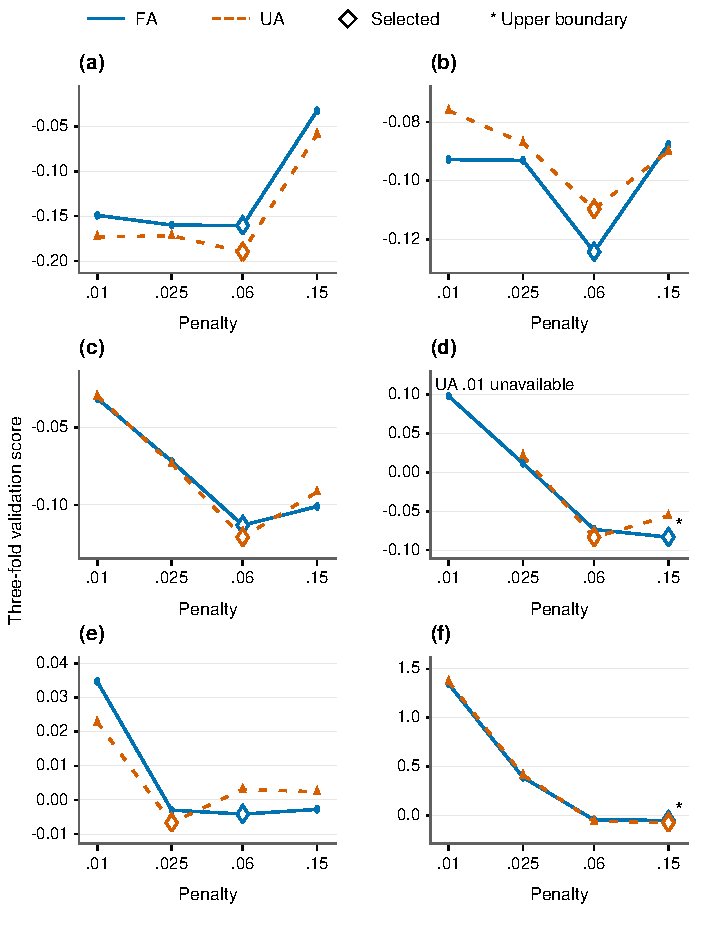
\includegraphics[width=119mm]{figures/Fig2.pdf}
 \caption{Training-only three-fold validation paths on S1--S6 in panels (a)--(f). FA uses solid lines and circles; UA uses dashed lines and triangles. Each score is the aggregate within-fold Gehan loss contrast against zero prediction; lower values are preferred. Diamonds mark selected penalties and asterisks mark the upper boundary of the original fixed grid. The S4 UA candidate at $\lambda=0.01$ has no aggregate score because one fold failed its numerical eligibility rule. Each panel uses one three-fold partition and its own vertical scale}
 \label{fig:cv-paths-local}
\end{figure}

Both methods select $\lambda=0.06$ in S1--S3 and $0.15$ in S6, with different choices in S4 and S5. Three selections are at the upper grid boundary. S4 fold 1 UA at $\lambda=0.01$ reaches the FISTA budget without satisfying the support-and-sign refinement gate, so that candidate has no aggregate score. At the selected penalties, FA has a lower validation score in S2, and UA has a lower score in S1 and S3--S6 (Table~\ref{tab:cv-model-summary}). The scores describe the stated training partitions.

The selected models reveal a structural distinction between residual sparsity and molecular prediction. In S4--S6, FA retains factor-mediated prediction with $\widehat{\bm{\beta}}=0$; its deployment slope has 300 exactly nonzero entries in every scenario. UA's deployment slope equals its molecular coefficient vector and shares its nonzero count (Table~\ref{tab:cv-model-summary}). These quantities summarize different roles in the fitted model: sparse residual effects and total molecular information in the frozen score.
\begin{table}[htbp]
\centering\small
\caption{Selected full-training models. $\|\hat{\bm{\beta}}\|_0$ counts exact nonzero penalized coefficients; $\|\hat{\bm{b}}_{\rm pred}\|_0$ counts exact nonzero frozen prediction slopes. CV is the three-fold score at the selected penalty; smaller is better. FISTA and Newton columns count accepted updates in the full-training refit}
\label{tab:cv-model-summary}
\setlength{\tabcolsep}{5pt}
\begin{tabular}{@{}llrrrrr@{}}
\toprule
Scenario & Method & CV & $\|\hat{\bm{\beta}}\|_0$ & $\|\hat{\bm{b}}_{\rm pred}\|_0$ & FISTA & Newton \\
\midrule
S1 & FA & -0.160420 & 58 & 300 & 449 & 0 \\
S1 & UA & -0.189698 & 55 & 55 & 314 & 0 \\
S2 & FA & -0.124238 & 36 & 300 & 209 & 0 \\
S2 & UA & -0.109671 & 38 & 38 & 1439 & 0 \\
S3 & FA & -0.113124 & 6 & 300 & 145 & 0 \\
S3 & UA & -0.120923 & 11 & 11 & 9178 & 0 \\
S4 & FA & -0.083292 & 0 & 300 & 0 & 0 \\
S4 & UA & -0.083487 & 7 & 7 & 7184 & 0 \\
S5 & FA & -0.004137 & 0 & 300 & 0 & 0 \\
S5 & UA & -0.006646 & 23 & 23 & 12054 & 0 \\
S6 & FA & -0.049824 & 0 & 300 & 0 & 0 \\
S6 & UA & -0.073506 & 2 & 2 & 1755 & 0 \\
\bottomrule
\end{tabular}
\end{table}


Nine UA fold candidates reach the prescribed accuracy after one qualified Newton update each. All twelve selected full-training fits finish without refinement. The S4--S6 FA refits satisfy the stopping test at their new nuisance initializations and take zero FISTA updates. Table~\ref{tab:cv-model-summary} reports refit work; Supplementary Appendix~\ref{app:reproducibility} includes initialization and complete work accounting.
\FloatBarrier
